\documentclass{beamer}
\mode<presentation>
\usepackage[utf8]{inputenc}
\usepackage{graphicx}
\usepackage[english,italian]{babel} % se non fosse inglese dovrei indicare la lingua nella quale sillabare [Italian]
%\usepackage{fancybox}
\usepackage{beamerthemeshadow}
\usepackage{ulem}
\usepackage{tikz}
\usepackage{fourier}

\usepackage{hyperref}
\hypersetup{
    colorlinks=true,
    linkcolor=blue,
    filecolor=magenta,      
    urlcolor=gter,
    pdftitle={Overleaf Example},
    pdfpagemode=FullScreen,
    }

\usetikzlibrary{snakes}
%\usepackage{beamertexpower}
%\beamertemplatetransparentcovereddynamicmedium
\usetheme{GTER} %(se vuoi mettere l'autore)
\useinnertheme{rectangles}
%\useoutertheme{infolines}
\usecolortheme[RGB={0,99,29}]{structure}
%\usecolortheme[RGB={0,99,29}]{palette quaternary}



\setbeamercovered{transparent}
\setbeamerfont{frametitle}{size=\small,series=\bfseries}
\definecolor{lightred}{rgb}{0.94,0.04,0.04}
\definecolor{aqua}{rgb}{0.00,0.80,1.00}
\definecolor{lightgreen}{rgb}{0.01,0.40,0.03}
\definecolor{limegreen}{rgb}{0.61,1.00,0.10}
\definecolor{peach}{rgb}{1.01,0.85,0.72}
\definecolor{purple}{rgb}{0.93,0.51,0.93}
\definecolor{indianyellow}{rgb}{0.98,0.75,0.30}
\definecolor{brick}{rgb}{0.70,0.13,0.13}
\definecolor{springsteen}{rgb}{0.00,0.49,0.19}
%%%%%%%%%%%%%%%%%%%%%%%%%%%%%%%%%%%%%%%%%%%%%%%%%%%%%%%%%%%%%%%%%%%%%%
\definecolor{gter}{rgb}{0.00,0.49,0.22} %verde GTER estratto da gimp
%%%%%%%%%%%%%%%%%%%%%%%%%%%%%%%%%%%%%%%%%%%%%%%%%%%%%%%%%%%%%%%%%%%%%%
\definecolor{lightorange}{rgb}{1.01,0.50,0.00}
\definecolor{royalblue}{rgb}{0.25,0.41,1.00}
\definecolor{lightgray}{rgb}{0.94,0.94,0.94}



\title{Principi di cartografia numerica}
\subtitle{I sistemi di riferimento}
\author[]{Gter srl Innovazione in geomatica Gnss e Gis}
%\author[]{Bianca Federici, Tiziano Cosso, \textbf{Roberto Marzocchi}, \\ Asimina Syriou}
\author[]{Relatore: Manuele Pesenti}
\date{Genova, settembre 2022}
\logo{
\includegraphics[height=0.5 cm]{./Gter.png}}


\begin{document}
{
%\setbeamertemplate{footline}{} 
\addtocounter{framenumber}{-1}  % non conto questa slide
\begin{frame}[plain]%[footline=false]
  \titlepage
  %\begin{center}
  			\begin{center}
  				
\includegraphics[height=1 cm]{./Gter.png}
  			\end{center}
  %\end{center}
\end{frame}
}

{

\section{Introduzione}

\subsection{L'importanza del Riferimento}

\begin{frame}
   \frametitle{L'importanza del Riferimento}

      \begin{center}
          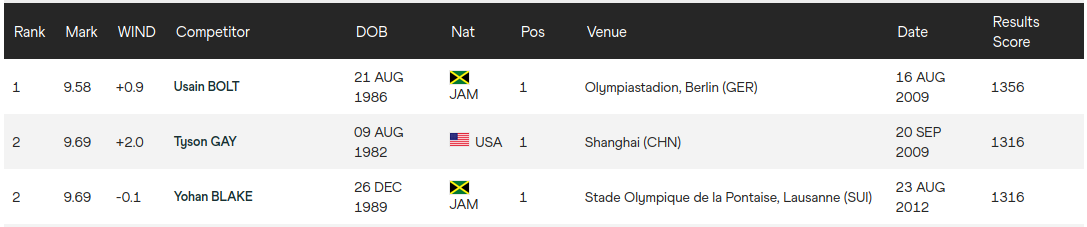
\includegraphics[width=1\textwidth] {./pics_2022_03/record100m.png}	
      \end{center} 
      Nella citta di Berlino nell'ambito dei campionati mondiali di atletica
      che si sono svolti il 16 agosto 2009 Il Sig. Usain Bolt ha impiegato
      9.58'' a percorrere 100 m su pista.
      \begin{columns}	
         	\begin{column} {0.5\textwidth}
            \begin{center}
                \textbf{A che ora} ha tagliato il traguardo?
            \end{center}
   		\end{column}
      		\begin{column} {0.5\textwidth}
   		   \begin{center}
               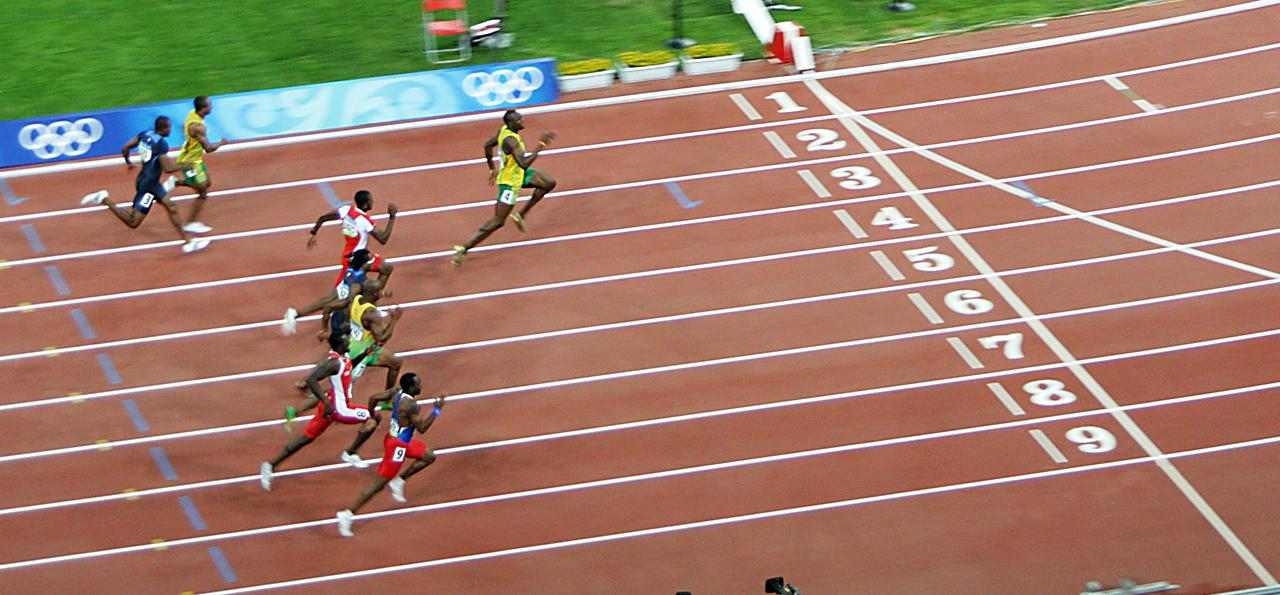
\includegraphics[width=1\textwidth] {./pics_2022_03/Usain_Bolt_winning-cropped.jpg}	
           \end{center} 
   		\end{column}
   	\end{columns}

\end{frame}

\begin{frame}
   \frametitle{L'importanza del Riferimento}

   \begin{itemize}
   		\item Cosa manca al quesito precedente?
   		\item L'informazione temporale fornita è espressa nel \textit{sistema locale} 
        del giudice di gara che ha sparato il colpo di inizio.
   		\item Nella richiesta è implicito un riferimento orario, presumibilmente:\\
            CET (Central European Time) UTC/GMT +1 hour (Berlin, Roma)
        \item Per poter rispondere devo poter applicare una \textbf{traslazione} del primo
        sistema sul secondo (\textbf{dato mancante})
   \end{itemize}

\end{frame}

\begin{frame}[allowframebreaks]
   \frametitle{Ma parliamo di GIS}
   \begin{center}
       \textsl{Professor Oleg McNoleg's guide to the successful use of Geographical
       Information Systems}
    \\( \textit{Ten ways to say nothing with GIS} )
   \end{center} 
    \href{https://teachgis.org/wp-content/uploads/2013/03/NoLeg_1998.pdf}
        {{\scriptsize int. j. geographical information science, 1998, vol. 12, no. 5, 429-430}}

    \begin{enumerate}
        \item [1] Never supply a map title, a \textbf{scale bar}, a \textbf{graticule},
      a \textbf{North arrow}, details of the \textbf{map projection} or a legend.\\
      \textit{This greatly reduces the chances that any map you produce can be misinterpreted}
      (Globus and Raible 1992).\\
      If you feel that the mapped region might still be recognizable then create the map
\textbf{using a Polar projection} (unless the study area is at one of the poles, in which
case use a \textbf{Mercator projection}). Clever use of colour and scale can also
detract from any information the map might still contain.

        \item [...]

        \item [4] Use as large a variety of \textbf{map scales} as possible.
        Scales are additive, the more scales are represented in your source data,
        the greater the range of scales that the output can be applied over.
        
        \item [...]
        
        \item [6] Do not waste your time checking your procedures.
        GIS are sophisticated tools designed to ensure that no invalid operations
        can be performed on the data by careless use.
        \textbf{It is therefore impossible to make a mistake}.
        Many GIS can now also co-register datasets automatically and with \textbf{infinite precision}.
        
    \end{enumerate}

\end{frame}

\begin{frame}
   \frametitle{Disclaimer}

      \begin{center}
          
\includegraphics[width=1\textwidth] {./pics_2022_03/index.jpeg}	
      \end{center} 

\end{frame}

\begin{frame}
   \frametitle{Tipologie di sistemi di riferimento nello spazio}
   Diverse sono le modalità per localizzare un certo luogo sul territorio, ossia i possibili \textbf{sistemi di riferimento}:
   \begin{columns}	
      	\begin{column} {0.2\textwidth}
			\begin{center}
				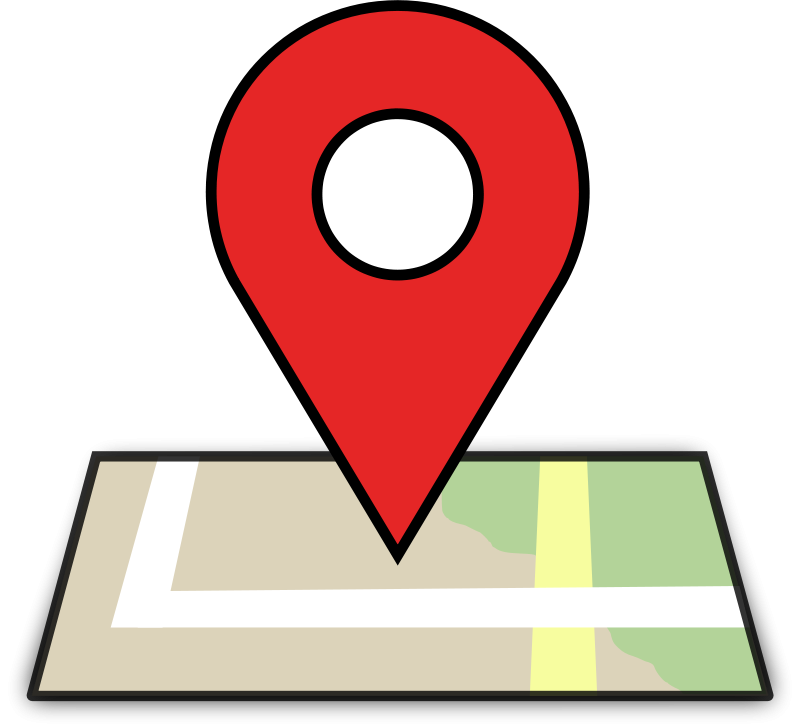
\includegraphics[width=1\textwidth] {./pics/location_icon.png}	
			\end{center} 
		\end{column}
   		\begin{column} {0.8\textwidth}
		   \begin{itemize}
		   		\item \textbf{Metrico}: definisce una posizione usando misure di distanza da una posizione fissata (origine).
		   		\item \textbf{Ordinato}: definisce la posizione in funzione della consequenzialità degli elementi (i numeri civici ordinano le case lungo le vie).
		   		\item \textbf{Toponomico}: definisce la posizione associando un nome ad un luogo (i nomi delle nazioni o delle città) 
		   \end{itemize}
		\end{column}
	\end{columns}

\end{frame}

\section{Georeferenziazione e GIS}

\begin{frame}
   \frametitle{Quanti sono i SR?}

   Alcuni numeri dall'\href{https://epsg.io/?q=}
        {\textbf{EPSG} \textit{Geodetic Parameter Dataset}}

   \begin{itemize}
        \item Projected (5486)
        \item Geodetic (925)
   \end{itemize}

{\small Con decine e decine di Sistemi di Riferimento usati in tutto il mondo, con la \textbf{necessità di scambiare informazioni cartografiche su scala globale} e con la diffusione dei software GIS, anche open source, si è resa necessaria una catalogazione di tutte queste informazioni per evitare confusione ed errori.\\
I sistemi di riferimento ed i relativi parametri di trasformazione sono stati codificati in registri mantenuti da organizzazioni mondiali.\\
Tra tutti questi registri, il più diffuso è il registro EPSG (\textbf{European Petroleum Survey Group}) attualmente gestito dal Comitato Geodetico dell'\textbf{International Association of Oil and Gas Producers} (OGP).

I codici EPSG sono ormai riconosciuti come standard per la classificazione dei Sistemi di riferimento in tutto il mondo. (\textsl{Fonte: \href{https://3dmetrica.it/i-codici-epsg/}
        {3dmetrica.it}})}

\end{frame}

\begin{frame}
   \frametitle{QGIS li ha tutti?}

         \begin{center}
      		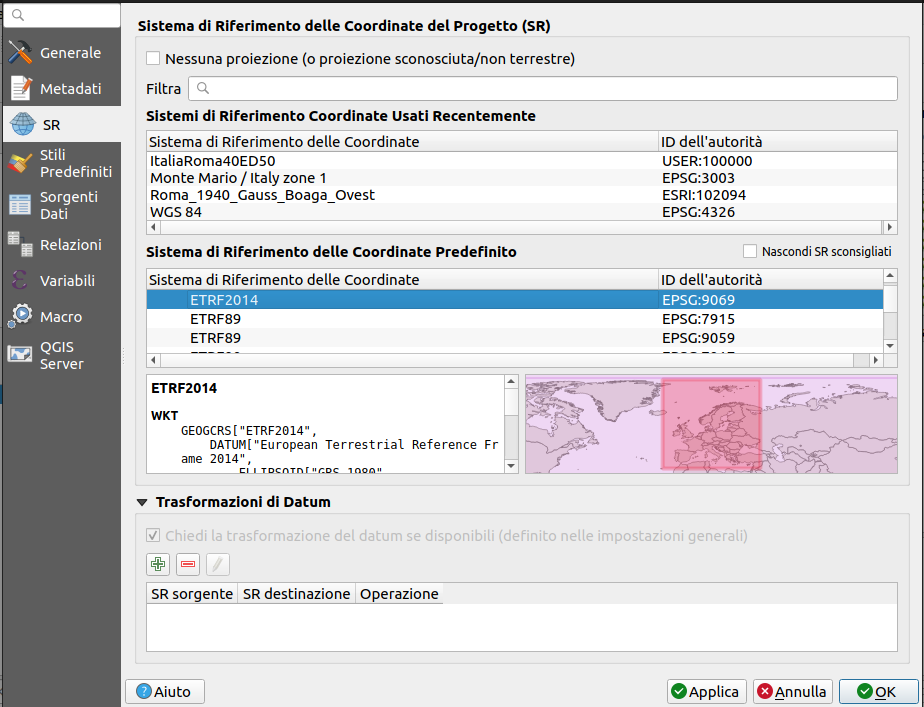
\includegraphics[height=.9\textheight, scale=1] {./pics_2022_03/qgis_sr.png}	
      	\end{center} 

\end{frame}

\section{Ma cosa è un SR?}

\begin{frame}
   \frametitle{Cosa tratta un GIS?}

   La componente geometrica di un GIS è composta da:
   \begin{itemize}
        \item Oggetti \textbf{vettoriali} cui è associata una serie di cooridnate;
        \item Oggetti \textbf{raster} di cui sono note la posizione geografica e
        l'estensione della cella
   \end{itemize}

   Per rappresentare le coordinate georeferenziate di un punto su una mappa occorre:
   \begin{itemize}
        \item determinare la posizione (assoluta o relativa) dei punti di intetresse appartenenti ad una porzine di superficie terrestre\\ (\textsl{Problema del rilievo});
        \item rappresentare i punti della superficie terrestre (irregolare e a doppia curvatura) su un supporto piano (la carta)\\ (\textsl{Problema della rappresentazione}).
   \end{itemize}

\end{frame}

\begin{frame}
   \frametitle{Cosa tratta un GIS?}

   I sistemi GIS dispongono di strumenti per la conversione di sistemi di riferimento
   ma è compito dell'utente:
   \begin{itemize}
        \item sapere se ha a che fare con dati basati su sistemi di riferimento diversi;
        \item sapere che la trasformazione applicata introduce errori che vanno
        ad alterare la scala nominale originale dei dati.
   \end{itemize}

   \begin{block}{Un esempio concreto}
        {\small Nei sistemi GNSS il dato viene rilevato rispetto al sistema WGS84 che è 
        diverso da quello (Roma40 / ED50) alla base della cartografia nazionale.} 
   \end{block}

   {\small Occorre fare in modo che più persone, rilevando porzioni di superficie terrestre
   diverse, diversi fenomeni nella stessa porzione o lo stesso fenomeno possano
   ottenere risultati \textbf{coerenti} e \textbf{confrontabili}}

\end{frame}

\begin{frame}
   \frametitle{Spoiler: Occorre distinguere}

    \begin{itemize}
         \item \textbf{Sistema di riferimento o \textit{Datum}}\\
            Insieme di \textbf{regole e misure} per la determinazione della posizione
            spazio temporale di un qualsiasi punto sulla Terra.\\
         
            % O ancora in maniera più rigorosa si può dire che è un insieme di misure
            % atte a fissare i gradi di libertà lasciati liberi da un insieme di misure.\\
            % (In questo caso si parla di \textit{Reference Frame} o realizzazione di un sistema di riferimento).
         
         \item \textbf{Sistema di coordinate}\\
            Rappresenta il modo con il quale viene espressa la posizione di un
            punto sulla superficie terrestre.
         
    \end{itemize}

\end{frame}

\begin{frame}
   \frametitle{Entriamo nel vivo}

   Coordinate cartesiane geocentriche\\
   (come quelle alla base dei sistemi GNSS)

    \begin{columns}	
          \begin{column} {0.4\textwidth}
          \begin{center}
              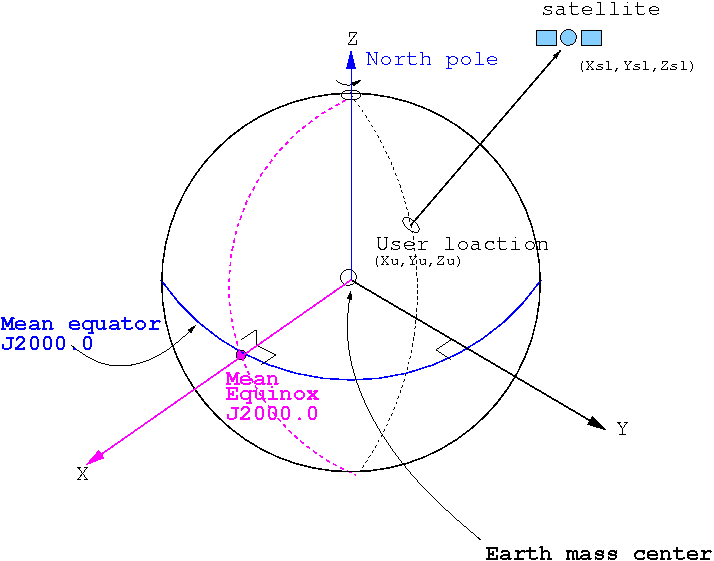
\includegraphics[width=\textwidth] {./pics_2022_03/CRS_reference_system.png}	
          \end{center}
          
      \end{column}
      \begin{column} {0.6\textwidth}
         \begin{itemize}
              \item 3 assi;
              \item una regola per le proiezioni ortogonali;
              \item 3 misure di distanza ($x, y, z$);
         \end{itemize}
      \end{column}
  \end{columns}

\end{frame}

\begin{frame}
   \frametitle{Entriamo nel vivo}

   Coordinate sferiche

    \begin{columns}	
          \begin{column} {0.4\textwidth}
          \begin{center}
              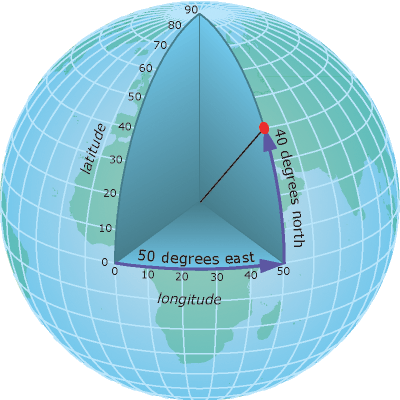
\includegraphics[width=\textwidth] {./pics_2022_03/latlon.png}	
          \end{center}
          
      \end{column}
      \begin{column} {0.6\textwidth}
         \begin{itemize}
              \item fisso una sfera di raggio noto;
              \item una regola per la misura della distanza dalla superficie di
              riferimento secondo la normale;
              \item 2 misure angolari e 1 di distanza ($\phi, \lambda, h$);
         \end{itemize}
      \end{column}
  \end{columns}

\end{frame}

\begin{frame}
   \frametitle{Entriamo nel vivo}

   Coordinate ellissoidiche o \textbf{geografiche}

    \begin{columns}	
          \begin{column} {0.4\textwidth}
          \begin{center}
              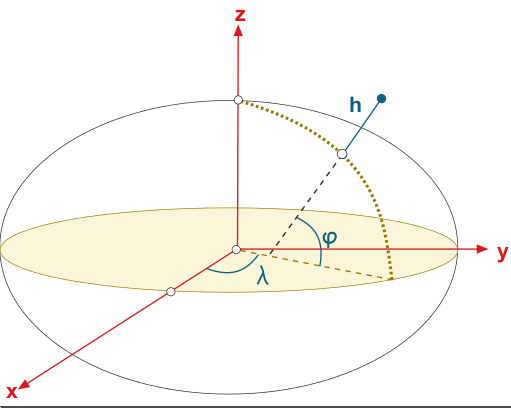
\includegraphics[width=\textwidth] {./pics_2022_03/Cartesian_Ellipsoid_Coord_coorenu.png}	
          \end{center}
          
      \end{column}
      \begin{column} {0.6\textwidth}
      
          Criteri simili a coordinate sferiche ma
          \begin{itemize}
              \item diversa superficie di riferimento
          \end{itemize}
          
          Geometrie di riferimento:
          \begin{itemize}
              \item asse di rotazione terrestre ($z$)
              \item centro di massa (origine)
              \item meridiano di riferimento di Greenwich (piano $xz$)
              \item equatore (piano $xy$)
          \end{itemize}
          
      \end{column}
  \end{columns}

\end{frame}

\begin{frame}
   \frametitle{Latitudine e longitudine}	
	
   \begin{columns}	
          \begin{column} {0.3\textwidth}
          \begin{center}
              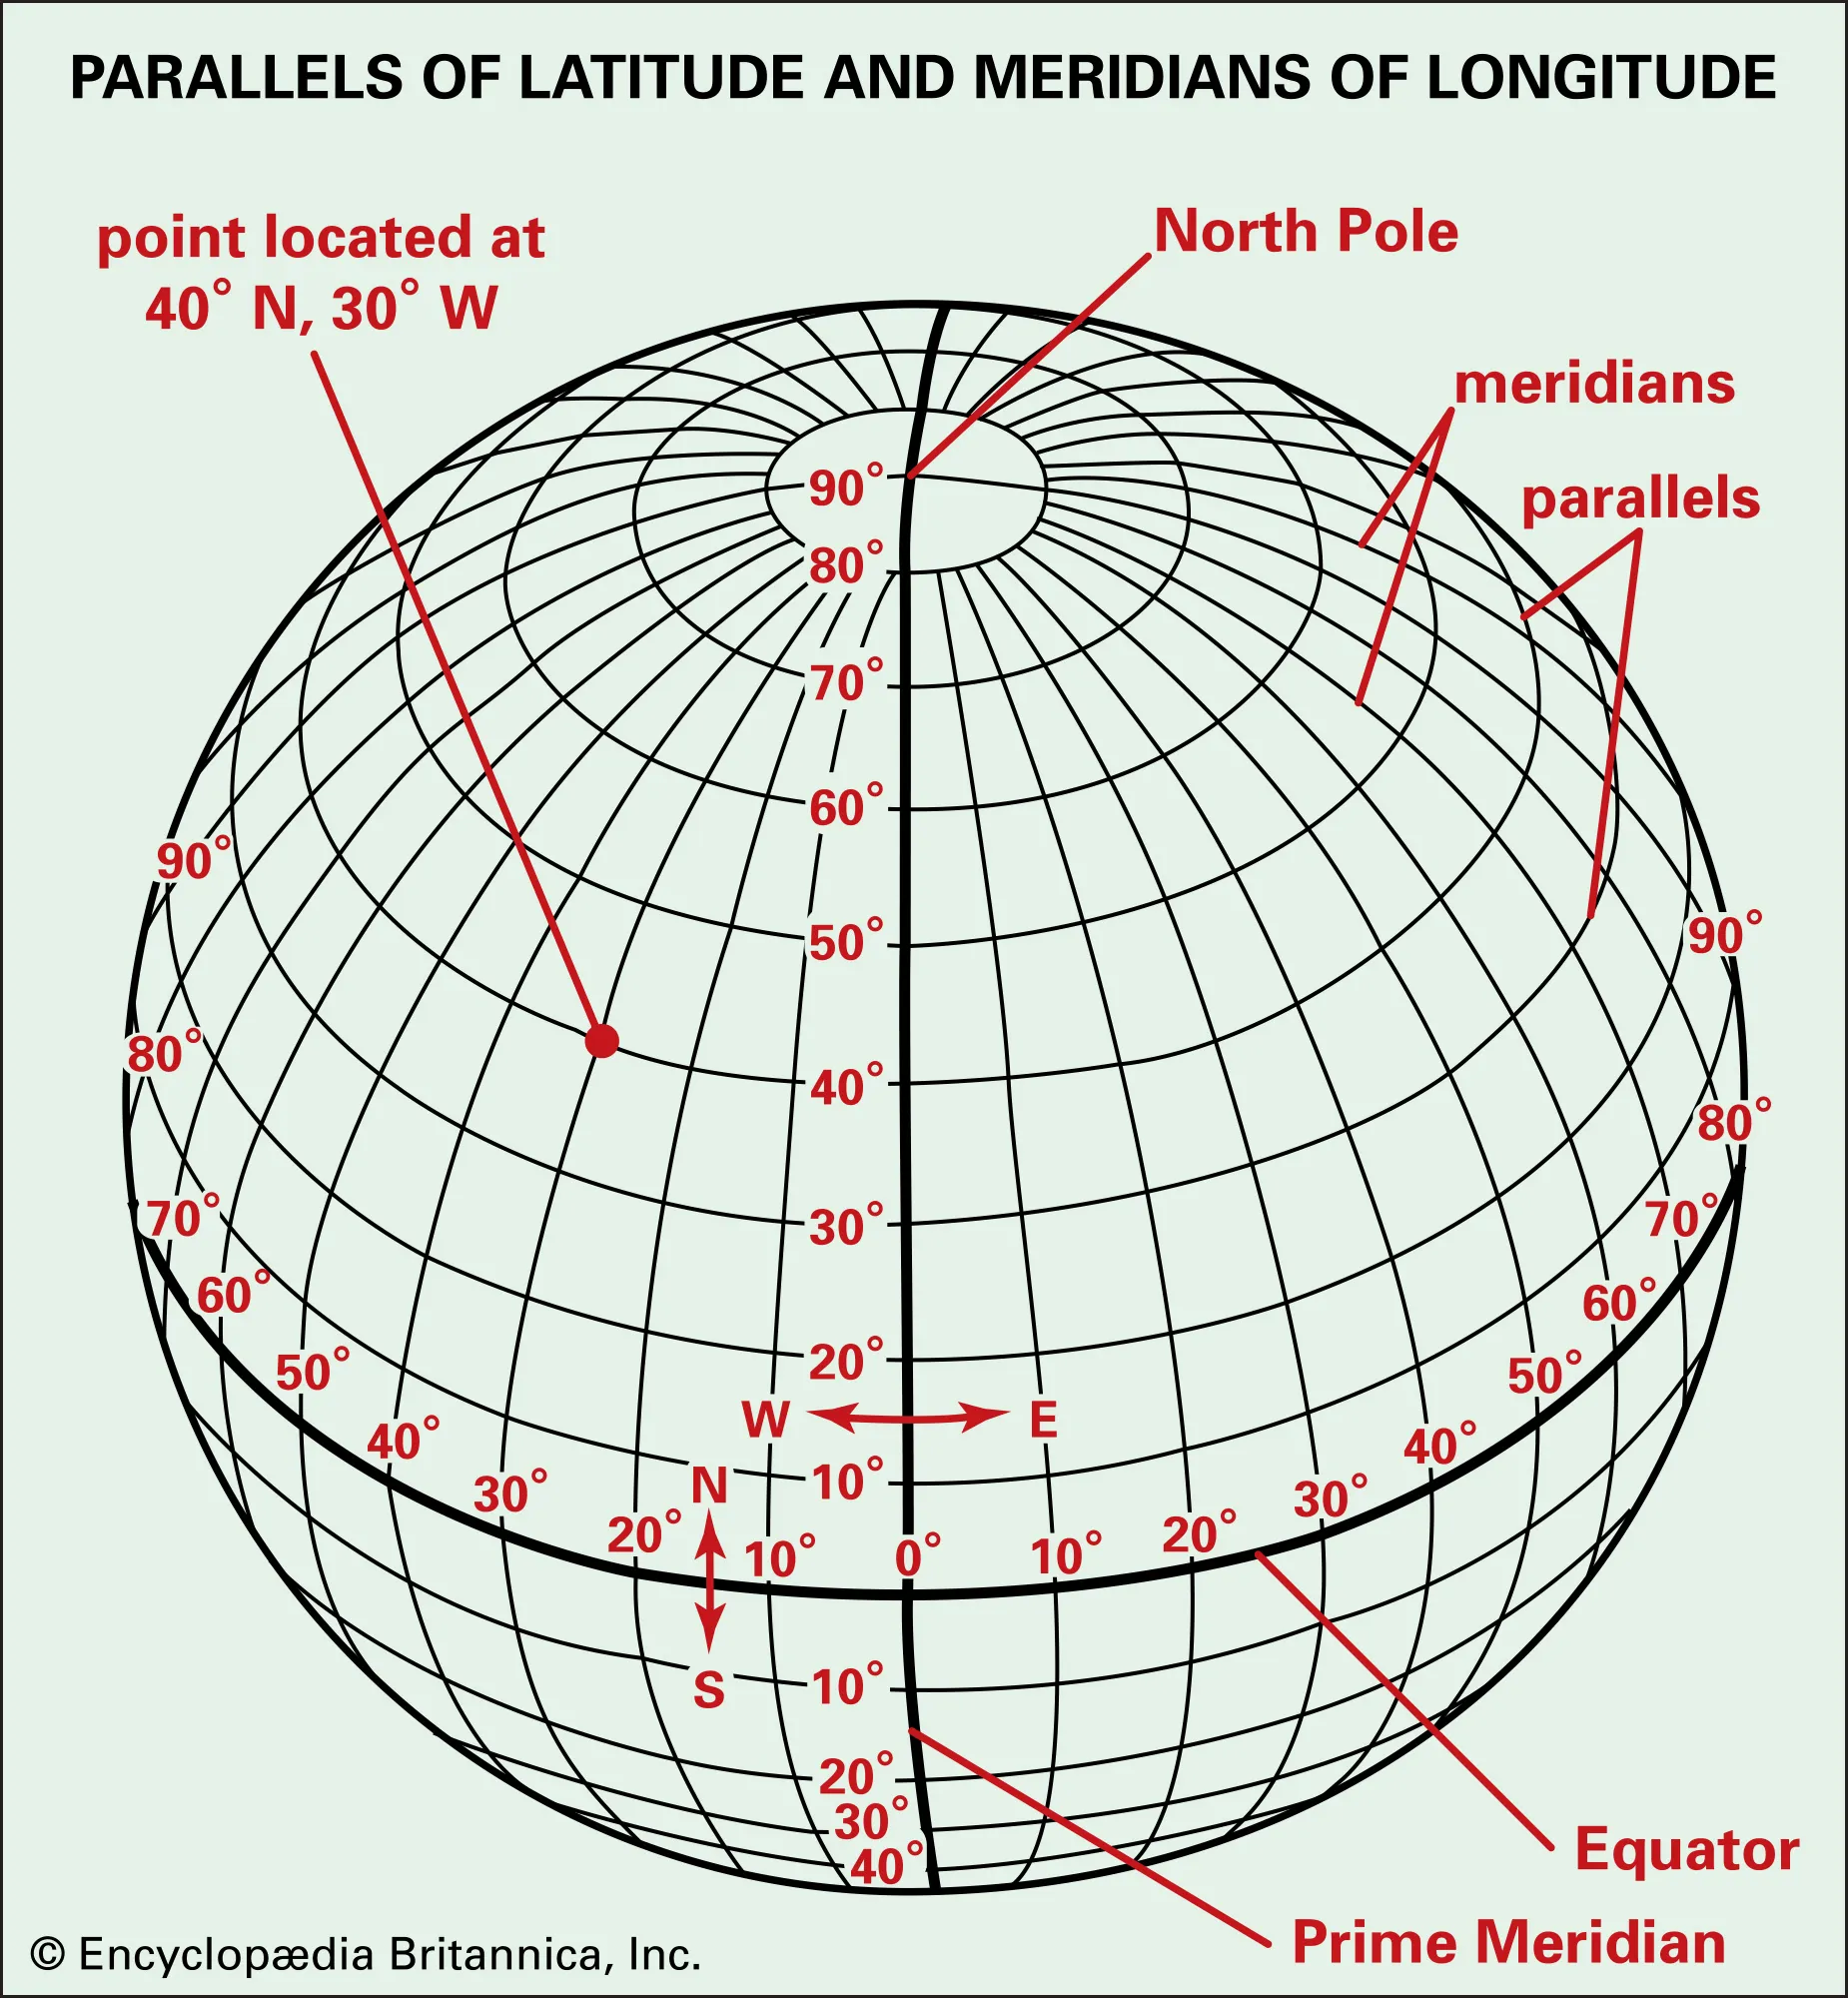
\includegraphics[width=\textwidth] {./pics_2022_03/meridiani_e_paralleli.png}	
          \end{center}
          
      \end{column}
      \begin{column} {0.7\textwidth}
      
          \begin{itemize}
      		\item latitudine $ \varphi $ \\
            {\scriptsize angolo fra il piano equatoriale e  la normale all'ellissoide per il punto}
      		\begin{center}
      		 $ -90^{\circ} \leq \varphi \leq +90^{\circ} $ \\
             $ 90^{\circ} S \leq  \varphi \leq 90^{\circ} N $ \\
             
             $ \varphi $ = cost.  $ \rightarrow $ parallelo
      		\end{center}
      		
      	    \item longitudine $\lambda$ \\
            {\scriptsize angolo lungo l'arco di parallelo tra il meridiano
            di Greenwich e quello passante per il punto}
          	\begin{center}
          		 $ -180^{\circ} \leq \lambda \leq +180^{\circ} $ \\
                 $ 180^{\circ} W \leq  \lambda \leq 180^{\circ} E $ \\
                 $ \lambda $ = cost.  $ \rightarrow $ meridiano
          		\end{center}
          	\end{itemize}
          
      \end{column}
  \end{columns}


\end{frame}

\begin{frame}
    \frametitle{Quale superficie di riferimento?}

    La qualità della rappresentazione geofrafica dipende dalla scelta di una
    superficie di riferimento

    \begin{columns}
        \begin{column}{0.7\textwidth}
        \begin{itemize}
            \item che approssimi al meglio la superficie fisica terrestre (manufatti compresi);
            \item sulla quale si possano proiettare i punti della superficie reale secondo la sua normale;
            \item che sia semplicemente esprimibile in termini matematici per effettuare
            calcoli parametrici (es. distanze, aree);
            \item per la quale la distanza misurata dalla superficie (quota) abbia un significato fisico; 
        \end{itemize}
            
        \end{column}
        \begin{column}{0.3\textwidth}
            \begin{center}
                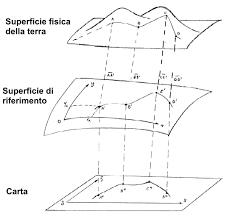
\includegraphics[width=\textwidth] {./pics_2022_03/refsup.png}	
            \end{center}
        \end{column}
        
    \end{columns}

\end{frame}

\begin{frame}
    \frametitle{Ma che forma ha la Terra?}

    La Terra ha la forma della Terra.
    
    \begin{block}{Il Geoide}
        \begin{itemize}
            \item Superficie equipotenziale nel campo della gravità che meglio
            approssima il livello medio del mare.
            \item Forma che assumerebbe il mare in condizione di equilibrio dinamico,
            in assenza di continenti e di influenze gravitazinali da parte della Luna
            e del Sole (maree).
            \item Superficie equipotenziale del campo di gravità terrestre passante
            per il livello medio marino di uno specifico punto sulla Terra, misurato
            con un mareografo su un tempo sufficientemente lungo in modo da eliminare
            l'effetto delle maree.
        \end{itemize}
    \end{block}

\end{frame}

\begin{frame}
    \frametitle{Ma che forma ha la terra?}

    \begin{columns}
        \begin{column}{0.5\textwidth}
            \begin{block}{Pregi}
                {\small \begin{itemize}
                    \item[\checkmark] \textbf{Fisicamente individuabile}: normale individuata dalle linee
                    di flusso del campo di gravità (materializzato dal filo a piombo)
                    \item[\checkmark] \textbf{Fisicamente significativa}: legata al moto dell'acqua
                    che tende a spostarsi verso quote geoidiche inferiori.
                \end{itemize}}
           \end{block}
        \end{column}
        \begin{column}{0.5\textwidth}
            \begin{center}
        		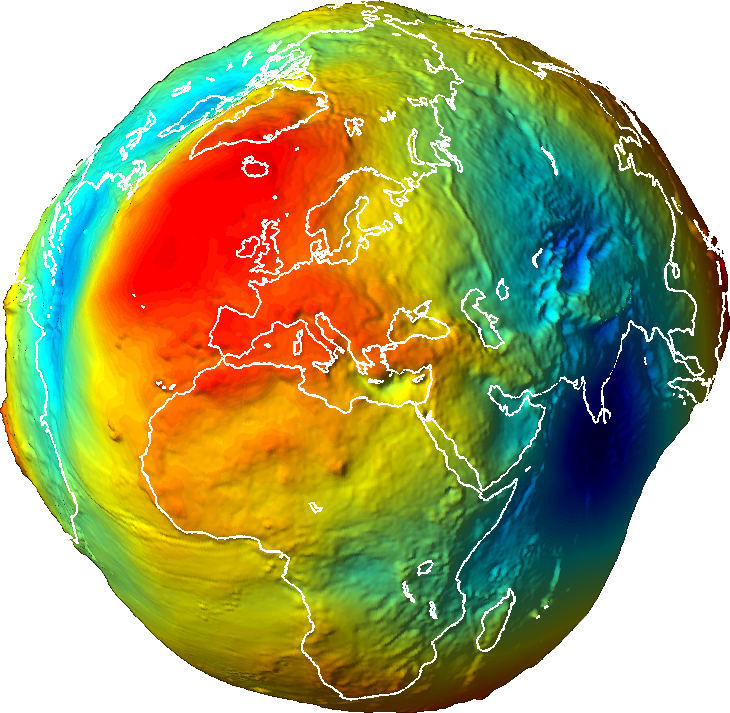
\includegraphics[width=\textwidth] {./pics/geoide.png}	
        	\end{center} 
        \end{column}
        
    \end{columns}

\end{frame}

\begin{frame}
    \frametitle{Ma che forma ha la terra?}

    \begin{columns}
        \begin{column}{0.5\textwidth}
            \begin{block}{Difetti}
                {\small \begin{itemize}
                    \item[\danger] non descrivibile con una formula matematica risolvibile;
                    \item[\danger] la direzione della forza di gravità dipende dalla \textbf{densità}
                        che la terra che assume in ogni punto\\
                        (impossibile da conoscere senza approssimazione);
                    \item[\danger] la definizione matematica del geoide è di fatto poco operativa;
                \end{itemize}}
           \end{block}
        \end{column}
        \begin{column}{0.5\textwidth}
            \begin{center}
        		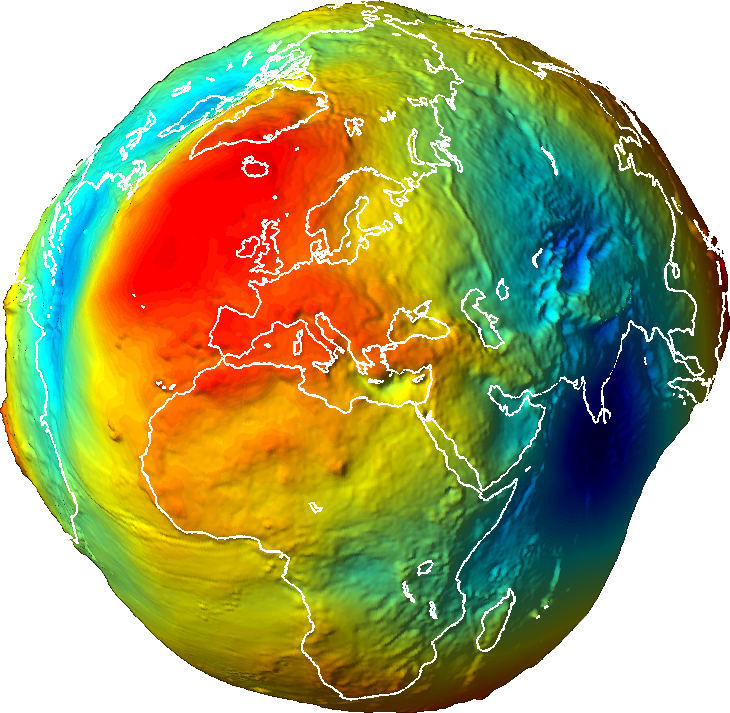
\includegraphics[width=\textwidth] {./pics/geoide.png}	
        	\end{center} 
        \end{column}
        
    \end{columns}

\end{frame}

\begin{frame}
    \frametitle{Una scelta difficile!}

    \begin{block}{Compromesso}
    In definitiva si adottano \textbf{due} riferimenti:
    \begin{itemize}
        \item \textbf{ellissoidico} (datum orizzontale o planimetrico) per stabilire
            latitudine e longitudine;
        \item \textbf{geoidico} (datum verticale o altimetrico) usato per le quote.
    \end{itemize}    
    \end{block}
    \begin{center}
        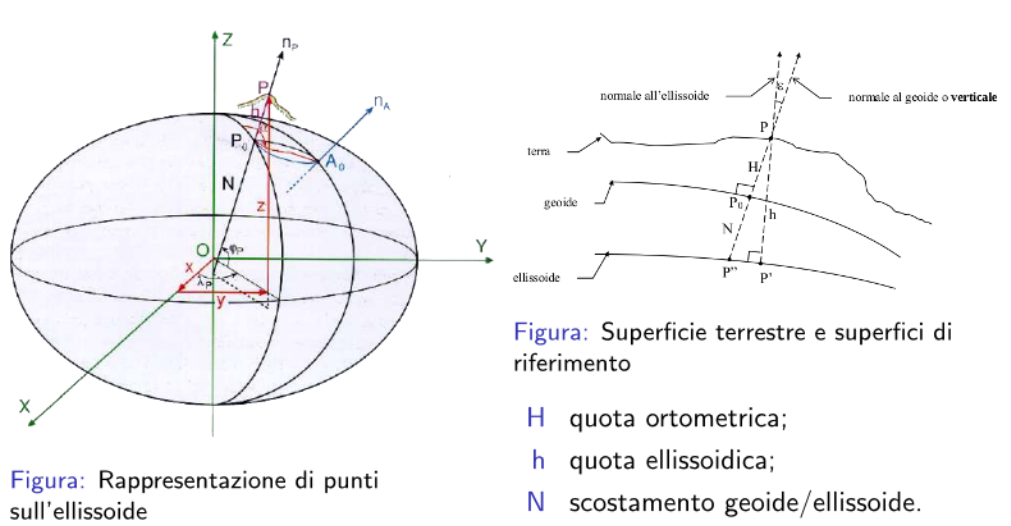
\includegraphics[height=.5\textheight]{./pics_2022_03/rifsups.png}	
    \end{center} 

\end{frame}

\begin{frame}
    \frametitle{Il compromesso}
    
    La scelta più ragionevole è quindi la terna ($\phi$, $\lambda$, $H$):
    {\small \begin{itemize}
        \item [$H$] \textbf{Quota ortometrica} misurata lungo le linee di forza 
            del campo gravitazionale terrestre rispetto alla superficie equipotenziale
            di riferimento (\textbf{geoide});
        \item[$\phi$, $\lambda$] \textbf{Coordinate ellissoidiche} rispetto all'ellissoide
            di rotazione prefissato:
            $$
            \frac{x^2+y^2}{a^2} + \frac{z^2}{b^2} = 1
            $$
    \end{itemize}}
    
    Quale ellissoide?!?... \textbf{dipende!}
    
    \begin{center}
        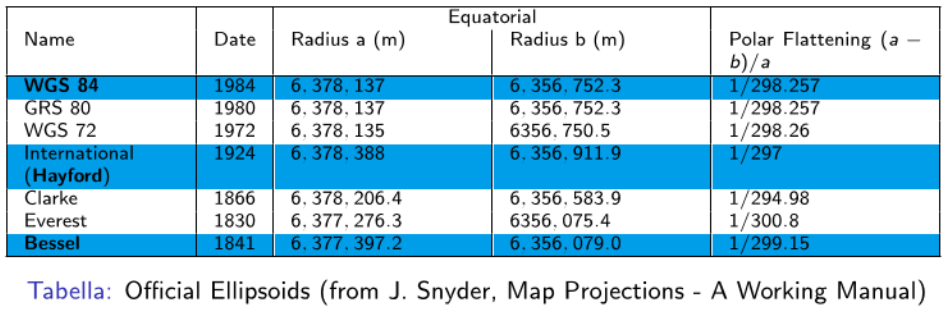
\includegraphics[height=.35\textheight]{./pics_2022_03/ellissoidi.png}	
    \end{center} 

\end{frame}

\begin{frame}
   \frametitle{Sistemi di riferimento altimetrico}
        Abbiamo quindi \textbf{due sistemi di riferimento altimetrico da non confondere}:
   \begin{itemize}
   		\item \textbf{quota ellissoidica}:lungo la perpendicolare all'ellissoide
		\item \textbf{quota ortometrica} (o geoidica): lungo la verticale fisica (filo a piombo)
   \end{itemize}
   \begin{center}
    	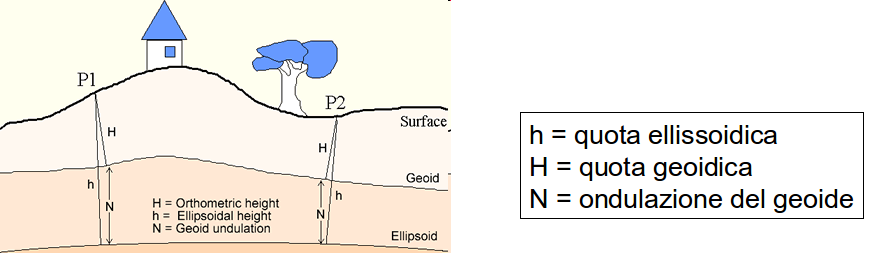
\includegraphics[width=1\textwidth] {./pics/altezze.png}
   \end{center}
\end{frame}

\begin{frame}
	\frametitle{Ellissoidi}
	Gli ellissoidi si distinguono anche dalla loro posizione e si distinguono in:
\begin{columns}	
	\begin{column} {0.3\textwidth}
	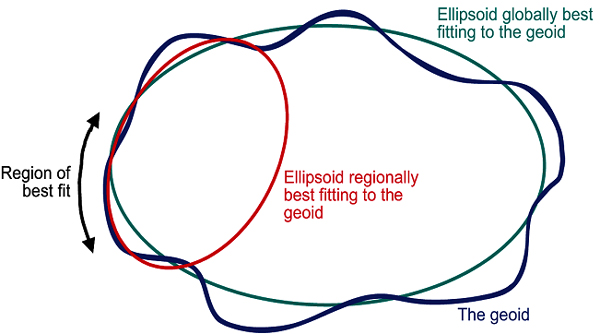
\includegraphics[width=1\textwidth] {./pics/ellissoide_locale_globale.jpg}	
	\tiny{Fonte: Knippers, 2002}
	\end{column}
	\begin{column} {0.7\textwidth}
		\begin{itemize}
            \item \textbf{Ellissoidi geocentrici}:\\
                {\scriptsize il centro geometrico dell'ellissoide coincide con il centro di massa
                e l'asse Z corrisponde all'asse medio di rotazione terrestre.\\
                (Adottati nel caso di sistemi di posizionamento satellitare GNSS)}
            
			\item \textbf{Ellissoidi locali}:\\
                {\scriptsize l'ellissoide viene posizionato tangente al geoide in un punto 
                convenzionale (detto \textit{punto di emanazione}).\\
                In questo caso:}
                \begin{itemize}
                    \item {\scriptsize il centro geometrico dell'ellissoide \textbf{non} è il centro di massa}
                    \item {\scriptsize l'asse Z \textbf{non} è l'asse di rotazione terrestre}
                \end{itemize}
		\end{itemize}
	\end{column}	
\end{columns}

\end{frame}

\section{cos'è un \textit{Datum}?}

\begin{frame}
   \frametitle{Datum}

   Lo abbiamo definito prima come:
   
   \begin{block}{\textit{Datum} geodetico}
       {\scriptsize Insieme di \textbf{regole e misure} per la determinazione della posizione
       spazio temporale di un qualsiasi punto sulla Terra.\\}
   \end{block}

   Ma quali regole e misure?
   
   \begin{block}{}
      Si intende l'insieme degli 8 parametri che definiscono la \textbf{forma}
      dell'ellissoide adottato ed il suo \textbf{orientamento}:
      \begin{itemize}
		\item {\scriptsize 2 parametri di forma dell'ellissoide (semiassi)}
		\item {\scriptsize 6 parametri di posizione e di orientamento}
		\begin{itemize}
			\item {\scriptsize latitudine e longitudine ellisoidica}
			\item {\scriptsize 2 componenti della deviazione della verticale}
            \item {\scriptsize altezza geoidica}
			\item {\scriptsize azimut ellisoidico}
		\end{itemize}
	\end{itemize}
   \end{block}

\end{frame}

\begin{frame}
    \frametitle{Frame}
    
    In altri termini matematici:
    
    \begin{block}{Realizzazione di un \textit{Datum}}
        L'insieme delle misure atte a fissare i gradi di libertà lasciati liberi
        da un insieme di misure.
    \end{block}

    \begin{columns}
        \begin{column}{0.68\textwidth}
            \begin{itemize}
                \item {\scriptsize si presenta come una lista di vertici, di cui vengono determinate le coordinate riferite a una certa epoca e la variazione di queste nel tempo (velocità).}
        		\item {\scriptsize si possono avere diverse realizzazioni dello stesso SR, in diversi tempi e con diverse modalità di misura con diversa precisione}
        		\item {\scriptsize la dinamica della crosta terrestre è il principale responsabile della variazione delle coordinate nel del tempo (pochi $mm$ o qualche $cm$ / $y$)}
            \end{itemize}
        \end{column}
        \begin{column}{0.32\textwidth}
            \begin{center}
                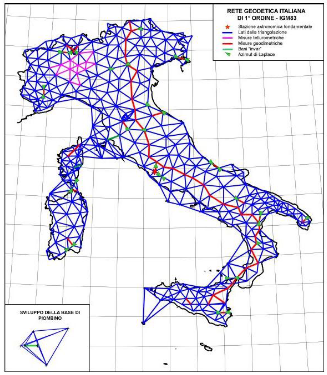
\includegraphics[width=1\textwidth] {./pics_2022_03/frame_Roma40.png}
            \end{center}
        \end{column}
        
    \end{columns}

\end{frame}

\begin{frame}
	\frametitle{Principali \textit{Frame}}

	\begin{itemize}
		\item \href{https://www.iers.org}{ITRS} e le sue realizzazioni ITRFxx
		\item ITRS e WGS84
		\item ITRS e le sue realizzazioni IGSxx
		\item \href{http://www.euref.eu/euref_egrs.html}{ETRS89} e le sue realizzazioni ETRFxx
		\item la materializzazione italiana RDN2008
	\end{itemize}
\end{frame}

\begin{frame}
	\frametitle{ITRFXX}
	\begin{itemize}
		\item Una realizzazione ITRF è legata ad una precedente (es. da ITRF89 a ITRF00) da una 	trasformazione di Helmert a 7 parametri (3 traslazioni , 3 rotazioni e 1 fattore di scala).
        I parametri di trasformazione variano linearmente nel tempo e definiscono ulteriori 7 parametri (3dt, 3dr, 1ds).
		\item Il passaggio successivo dalla realizzazione ITRF iniziale ad un'epoca generica (es. da 	ITRF00(00) a ITRF00(08)) avviene secondo un modello lineare
	\end{itemize}

\end{frame}

\begin{frame}
	\frametitle{WGS84}
	\begin{itemize}
		\item Originariamente, il SR WGS84 è stato realizzato nel 1987 con misure Doppler (Sistema NNSS o Transit).
		\item Le prime realizzazioni del WGS84 coincidevano con ITRS entro tolleranze di un metro.
		\item Le realizzazioni recenti del WGS84 sono basate anch'esse su misure GPS.
		\item Le realizzazioni recenti del WGS84 (G730 del 1994, G873 del 1996/7 e G1150 del 2001) coincidono praticamente con il corrispondente ITRF entro un margine di circa 10 cm.
	\end{itemize}
	
\end{frame}

\begin{frame}
	\frametitle{IGS}
		\begin{itemize}
		\item L'International GNSS Service (IGS) riunisce oltre 200 agenzie nel mondo (Nasa, IGN...) al fine di condividere risorse e dati GPS e GLONASS per fornire prodotti GPS e GLONASS di elevata precisione (effemeridi, coordinate stazioni, parametri iono e troposferici, movimenti del polo etc) .
		\item IGS è un servizio dell' International Association of Geodesy (IAG) e raccoglie i dati di 420 stazioni GNSS mondiali, di cui oltre 350 attive
		\item IGS opera per migliorare la definizione dell'ITRS.
		\item \textbf{Le soluzioni IGS sono più indicate per le applicazioni GNSS}
	\end{itemize}	
\end{frame}

\begin{frame}
	\frametitle{ETRS89}
	\begin{itemize}
		\item ETRS - European Terrestrial Reference System
		\item Le coordinate ITRF variano nel tempo: da mm a cm/anno. Ciò è dovuto ai movimenti delle 	placche. Per ridurre questo effetto si considera un SR solidale alla placca europea: origine e orientamento
		degli assi si muovono rigidamente con essa.
		\item \textbf{ITRF e ETRF coincidono all'anno 1989} (ITRS89=ETRS89).
	\end{itemize}	
\end{frame}



\begin{frame}
	\frametitle{RDN2008}
	Il sistema di riferimento ufficiale è ora costituito dal Datum RDN2008. In particolare la rete di raffittimento RDN 2008 costituisce la realizzazione del SR ETRF2000 epoca 2008.0, realizzazione del sistema globale ETRS89 adottato dall'Europa (\textit{divenuto obbligatorio a livello nazionale in seguito del DM 10 novembre 2011})

	In particolare l' European Terrestrial Reference System 1989:	
	
	\begin{itemize} 
		\item usa l'ellissoide GRS80
		\item è un sistema di riferimento cartesiano geodetico di tipo di ECEF (Earth-centred, Earth-fixed, cioè geocentrico), dove la placca Eurasiatica è statica. In Europa, le coordinate e le mappe basate sull'ETRS89 non sono soggette al cambiamento causato della deriva continentale. È il datum ufficiale adottato in Europa.
	\end{itemize}
	
\end{frame}



\begin{frame}
   \frametitle{Datum definiti per l'Italia}
   \begin{columns}	
		\begin{column}{0.8\textwidth}
			
            \begin{itemize}
                \item \textbf{Roma40} Adottato in Italia a partire dal 1940:
                \begin{itemize}
                    \item ellissoide Internazionale 1924 (Hayford)
                    \item orientato sul caposaldo geodetico di \href{https://www.openstreetmap.org/search?whereami=1\&query=41.92441\%2C12.45212\#map=14/41.9246/12.4521}{Roma Monte Mario}
                \end{itemize}
                \item \textbf{GRS80}
                \item \textbf{Rif. Catastale}
                \begin{itemize}
                    \item ellissoide Bessel
                    \item orientato a Genova all'\href{https://www.openstreetmap.org/search?whereami=1\&query=44.4195\%2C8.9213\#map=16/44.4195/8.9213}{Istituto Idrografico della Marina}
                \end{itemize}
            \end{itemize}
            
            
		\end{column}
        \begin{column}{0.2\textwidth}
    		
\includegraphics[width=1\textwidth] {./pics/ita.jpg}
		\end{column}	
	\end{columns}

\end{frame}

\begin{frame}
\frametitle{Datum utilizzati in Italia}

Ma \textbf{quanti} e \textbf{quali} sono i \textit{datum} usati in Italia?

\begin{itemize}
	\item ETRF2000 (RDN 2008): Realizzazione italiana del sistema globale ETRS89
	\item ETRF89/ETRS89	
	\item ED50	 
	\item Roma40 Monte Mario
	\item WGS84
\end{itemize}

\begin{center}
e le proiezioni?!?!?
\end{center}
\end{frame}

\section{Proiezioni}

\begin{frame}
   \frametitle{Proiezioni}
	La superficie della terra è curva,ma ci sono molte ragioni che ci spingono a
    rappresentarla su piano anche la cartografia numerica.
	\begin{itemize}
		\item La carta utilizzata per rappresentare i risultati di analisi fatte col GIS è piatta.
		\item Le carte piatte sono scansionate ed utilizzate per creare dati GIS.
		\item Il modello raster è piatto
		\item Non si può vedere contemporaneamente tutta la terra su una superficie curva.
		\item È molto più facile effettuare misure nel piano (aree, distanze, direzioni).
	\end{itemize}
	Per questa ragione anche in cartografia numerica si utilizzano le diverse proiezioni cartografiche.
\end{frame}

\begin{frame}
   \frametitle{Proiezione cartografica}
	\begin{center}
	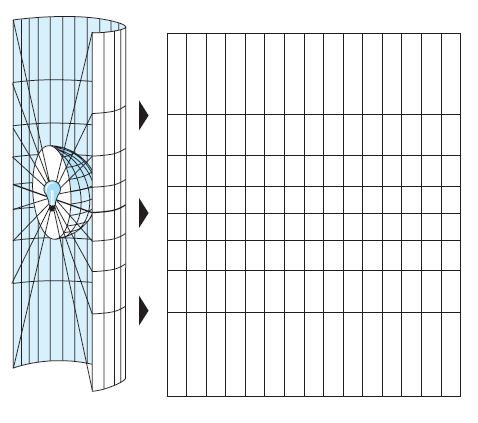
\includegraphics[width=0.8\textwidth] {./pics/proiezione.png}
	\end{center}
\end{frame}

\begin{frame}
   \frametitle{Tipi di proiezione}
	Le proiezioni cartografiche trasportano coordinate dall'ellissoide del sistema di riferimento al piano della carta. \textbf{Le due superfici non sono topologicamente equivalenti, quindi \textcolor{red}{non} è possibile passare da ellissoide a carta senza deformazioni.} \\
	\bigskip
    È possibile però nel passaggio tra ellissoide e piano della carta porsi
    degli obiettivi (ma solo uno per volta!!):
	\begin{itemize}
		\item conservare gli angoli $\rightarrow $ \textit{carta conforme}
		\item conservare le superfici $\rightarrow $ \textit{carta equivalente}
		\item minimizzare tutte le deformazioni, senza annullarne nessuna $\rightarrow $  \textit{carta afilattica}
	\end{itemize}
\end{frame}

\begin{frame}
   \frametitle{Tipi di proiezione}
	A seconda del tipo di forma usato per effettuare le proiezioni si distinguono: 
	\begin{itemize}
		\item \textit{proiezioni piane}
		\item \textit{proiezioni cilindriche}
		\item \textit{proiezioni coniche}
	\end{itemize}
\end{frame}

\begin{frame}
   \frametitle{Proiezioni piane}
	\begin{center}
		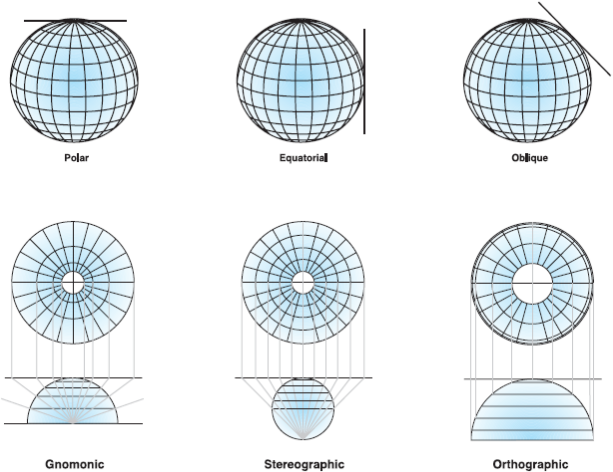
\includegraphics[width=0.8\textwidth] {./pics/piane.png}
	\end{center}
\end{frame}

\begin{frame}
   \frametitle{Proiezioni cilindriche}
	\begin{center}
		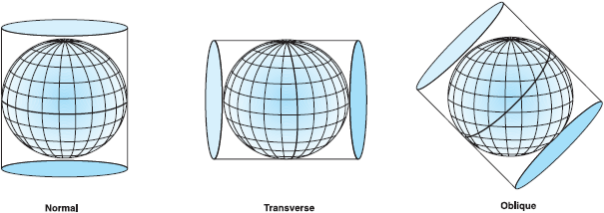
\includegraphics[width=0.8\textwidth] {./pics/cilindriche.png}
	\end{center}
\end{frame}

\begin{frame}
   \frametitle{Proiezioni coniche}
	\begin{center}
		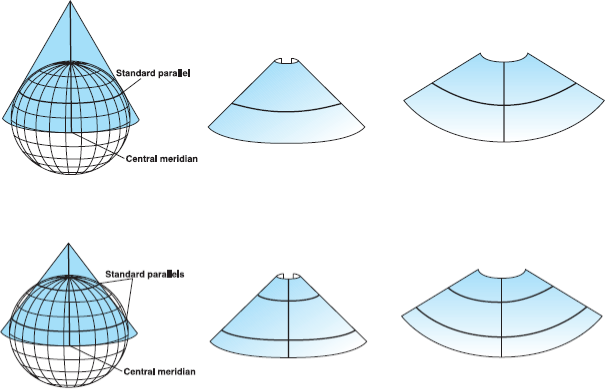
\includegraphics[width=0.8\textwidth] {./pics/coniche.png}
	\end{center}
\end{frame}

\begin{frame}
   \frametitle{Proiezioni usate in Italia}
Ci sono moltissimi tipi di proiezioni cartografiche, quelle storicamente utilizzate in Italia sono:
	\begin{itemize}
		\item UTM (Universal Trasversal Mercator), utilizzata a livello mondiale
		\item Gauss-Boaga, utilizzata per il datum Roma 40 Monte Mario 
		\item Cassini-Soldner, utilizzata dal Nuovo Catasto dei Terreni italiano 
	\end{itemize}
	\begin{center}
		
\includegraphics[width=0.2\textwidth] {./pics/ita.jpg}
	\end{center}
\end{frame}

\begin{frame}
   \frametitle{Proiezione UTM}
	\small
	\begin{itemize}
		\item Un tipo di proiezione \textbf{cilindrica}
		\item \textbf{Trasversa di Mercatore} perché il cilindro è tangente aipoli e non all’equatore
		\item è \textbf{conforme} (conserva gli angoli)
		\item Usa un sistema di \textbf{60 zone} (o fusi) di ampiezza pari a $ 6^{\circ}$ e distorsione massima del 0.04 \%
		\item il meridiano centrale è reso con un fattore di contrazione 0.9996 e ha modulo di deformazione costante
		\item meridiani e paralleli sono resi come rette perpendicolari tra loro
		\item è simmetrica rispetto all’equatore
		\item per avere coordinate sempre positive su ogni fuso, la coordinata Est (misurata dal meridiano centrale) ha una falsa origine pari a
500000 m 
		\item la proiezione è limitata tra gli $ 80^{\circ} S $ e gli $ 80^{\circ} N $
	\end{itemize}
\end{frame}


\begin{frame}
   \frametitle{Proiezione UTM}
	\begin{center}
		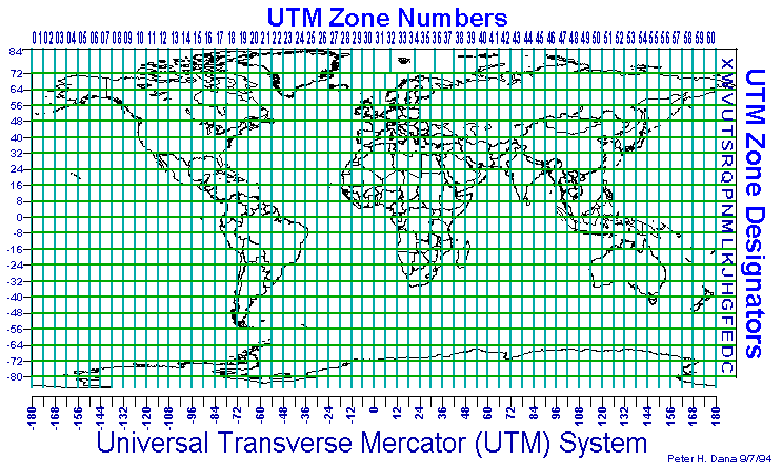
\includegraphics[width=1\textwidth] {./pics/utm_zones.png}
	\end{center}
\end{frame}

\begin{frame}
   \frametitle{Proiezione UTM}
	Utilizzato come tipo di proiezione internazionale standard da:
	\begin{itemize}
		\item datum europeo ED50;
		\item datum europeo ETRS89; 
		\item datum internazionale WGS84;
		\item materializzazione italiana IGM95 e ETRF2000.
	\end{itemize}
\end{frame}

\begin{frame}
   \frametitle{Proiezione Gauss Boaga }
	\small
	\begin{itemize}
		\item Un tipo di proiezione \textbf{cilindrica} di gauss (proiezione inversa di mercatore)
		\item la proiezione viene fatta su due fusi, indicati come fuso Ovest ed Est, di ampiezza di $ 6^{\circ} 30'$ corrispondenti all'incirca ai fusi UTM 32 e 33
		\item il meridiano centrale è reso con un fattore di contrazione 0.9996 per avere coordinate sempre positive su ogni fuso, la coordinata Est ha una falsa origine pari a 1500000 m sul fuso Ovest e 2520000 m sul fuso Est
		\item il fuso Ovest si estende da $6^{\circ}$ a ovest di Greenwitch a $ 12^{\circ} 30'$ , con meridiano centrale a $ 9^{\circ}$
		\item il fuso Est si estende da $ 12^{\circ} 30'$  a ovest di Greenwitch a $ 18^{\circ} 30'$ con meridiano centrale a $ 15^{\circ}$
		\item i due fusi sono quindi sovrapposti per circa $ 1^{\circ}$ per facilitare il passaggio tra i due fusi e il fuso Est è esteso di altri 30' per comprendere la zona più ad est della Puglia
	\end{itemize}
\end{frame}

\begin{frame}
   \frametitle{Proiezione Gauss Boaga}
	\begin{center}
		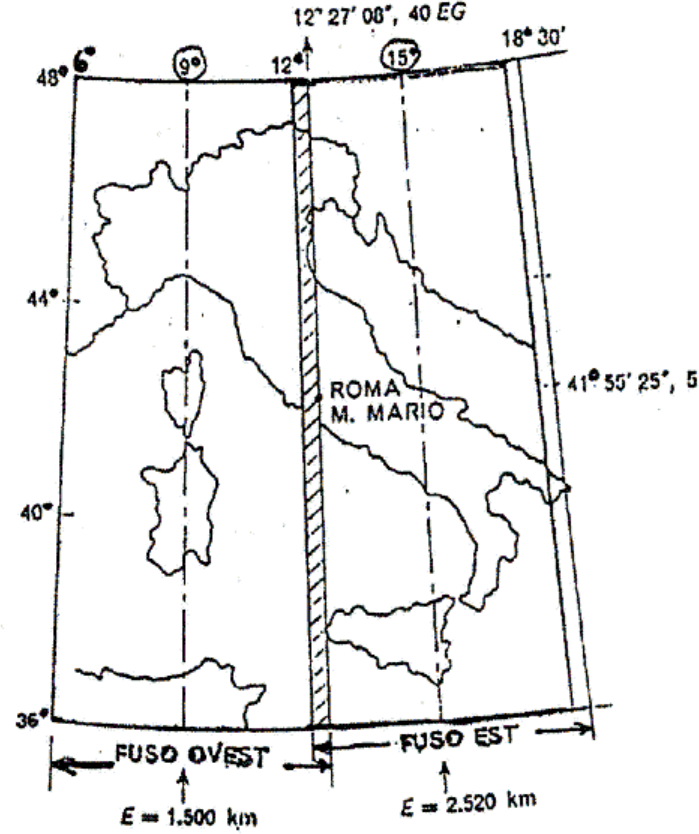
\includegraphics[width=0.55\textwidth] {./pics/GB.png}
	\end{center}
\end{frame}

\begin{frame}
\frametitle{Suddivisione in fusi "standard"}
Per molte regioni per esempio la suddivisione proposta dai fusi Gauss Boaga (Est/Ovest) o UTM (32, 33 e 34 N) va benissimo.
\begin{center}
	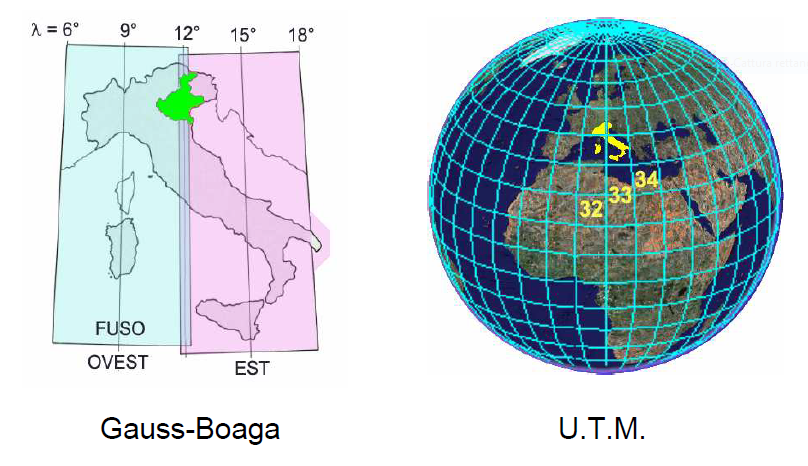
\includegraphics[width=0.75\textwidth] {./pics/proiezioni0.PNG}
\end{center}
\end{frame}

\begin{frame}
\frametitle{Fuso Italia}
 \begin{columns}
 	\begin{column} {0.65\textwidth}
 		\begin{center}
 			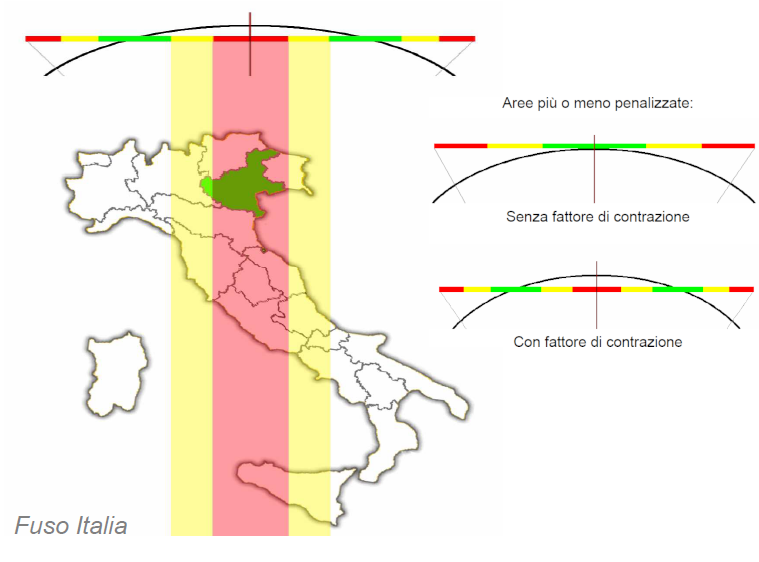
\includegraphics[width=1\textwidth] {./pics/proiezione1_FI.PNG}
 		\end{center}
 	\end{column}
	\begin{column} {0.35\textwidth}
		Si è poi definita una proiezione (Fuso Italia) che introduce un fattore di contrazione per minimizzare le deformazioni sull'intero territorio nazionale
	\end{column}
 \end{columns}
\end{frame}

\begin{frame}
\frametitle{Fuso 12}
 \begin{columns}	
	\begin{column} {0.5\textwidth}
		E infine, Regione Veneto che come altre regioni risulta a cavallo fra i fusi UTM e al contempo penalizzata dalla definizione del fuso Italia e dal fattore di contrazione, ha proposto un’ulteriore proiezione (Fuso 12) in grado di minimizzare le deformazioni su tutto il suo territorio.
	\end{column}
\begin{column} {0.5\textwidth}
\begin{center}
	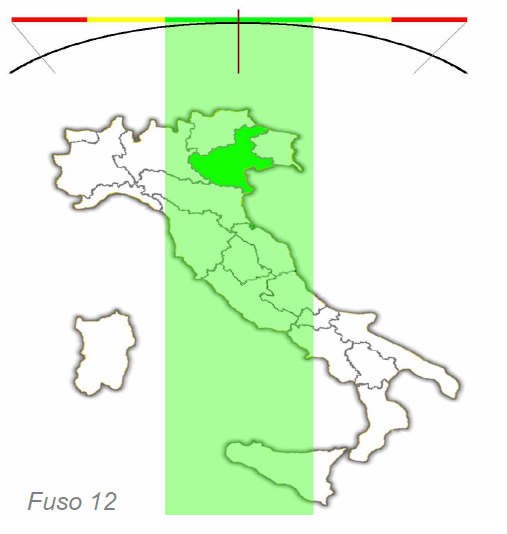
\includegraphics[width=1\textwidth] {./pics/proiezione2_F12.PNG}
\end{center}
\end{column}
\end{columns}
\end{frame}

\begin{frame}
   \frametitle{Sistema di riferimento}
   In definitiva la definizione di un sistema di riferimento è così data:
    \begin{itemize}
   		\item \underline{\textbf{sistemi di coordinate geografiche}}
		\begin{center}
			\textbf{datum}
			\\(\textit{es. WGS84, Roma40, Monte Mario})
		\end{center}
   		\item \underline{\textbf{sistemi di coordinate proiettate}}
 		\begin{center}
			\textbf{datum + sistema di proiezione}
			\\(\textit{es. WGS84-UTM32N \\ Roma 40 Monte Mario - Gauss Boaga Fuso Ovest})
		\end{center}  		
   	\end{itemize}
\end{frame}

\begin{frame}
   \frametitle{I registri di parametri geodetici}
   
    \begin{itemize}


%  	\item Le definizioni dei sistemi di riferimento e i parametri di trasformazione utilizzati da quasi tutti i GIS sono definiti tramite le \textbf{librerie  \href{http://trac.osgeo.org/proj/}{\textcolor{gter}{\emph{proj4}}}}.
%  	\begin{center}
%  	
\includegraphics[width=0.2\textwidth] {./pics/proj_logo.png}
%  	\end{center}
  	\item Inoltre tutti i GIS utilizzano i registri di parametri geometrici di cui il più conosciuto è quello rappresentato dai \textbf{codici EPSG} (European Petroleum Survey Group) per definire in maniera univoca i vari sistemi di riferimento mondiali.
  	
  \end{itemize}	
   
\begin{center}
   \href{http://spatialreference.org/}{\textcolor{gter}{\emph{http://spatialreference.org/}}}
\end{center}

\end{frame}

\begin{frame}
   \frametitle{Codici EPSG in Italia}
  \footnotesize
     \begin{columns}	
		\begin{column} {0.4\textwidth}
    		
   \textbf{Sist. coordinate geografiche}:
   \footnotesize{	
    \begin{itemize}
    	\item WGS84$\rightarrow$EPSG 4326
    	\item ETRF2000(RDN2008) $\rightarrow$EPSG 6706
    	\item ETRF89/ETRS89 $\rightarrow$EPSG 4258
    	\item ED50$\rightarrow$EPSG 4230
    	\item Roma40 (o Monte Mario):
    	\begin{itemize}
    		\item EPSG 4265 \tiny{longitudini rispetto a Greenwich}
    		\item \footnotesize{EPSG 4806} \tiny{longitudini rispetto a M. Mario}
   	 	\end{itemize}  	
  	\end{itemize}
  	}
  	\end{column}
	\begin{column} {0.6\textwidth}
  	
    \textbf{Sist. coordinate cartografiche}:
    \footnotesize{		
    \begin{itemize}
		\item WGS84-UTM32/33N$\rightarrow$EPSG 32632/33
		%\item WGS84-UTM33N $ \rightarrow $ EPSG 32633
		%\\..
		\item ED50-UTM32/33N$\rightarrow$EPSG 23032/33
		%\item ED50-UTM33N $ \rightarrow $ EPSG 23033
		%\\..
		\item ETRS89-UTM32/33N$\rightarrow$EPSG 25832/33
		%\item ETRS89-UTM33N $ \rightarrow $ EPSG 25833
		%\\..
		\item Roma40-GB F. OVEST$ \rightarrow $EPSG 3003
		\item Roma40-GB F. EST$ \rightarrow $EPSG 3004
		\item RDN2008-UTM32N$\rightarrow$EPSG 7791 (6707)
		\item RDN2008-UTM33N$\rightarrow$EPSG 7792 (6708)
		\item RDN2008-UTM34N$\rightarrow$EPSG 7793 (6709)
		\item RDN2008-F. Italia$\rightarrow$EPSG 7794 (6875)
		\item RDN2008-Zona12$\rightarrow$EPSG 7795 (6876)
					
  	\end{itemize}
	}
  	\end{column}
  	\end{columns}
%  	\bigskip 
%  	Nota: La materializzazione del nostro sistema ETRF2000 inficia solo le trasformazioni di alta precisione (e quindi i grigliati), per cui in ambiente GIS i  parametri da usare generalmente sono gli stessi che si usano per WGS84. 

\end{frame}

\begin{frame}
   \frametitle{Le coordinate di Genova...}
  Abbiamo detto che Genova ha le seguenti coordinate \textbf{geografiche:}
			\begin{itemize}
				\item $ 44^{\circ} 24' 40.16 N $
				\item $ 08^{\circ} 55' 57.58 E $
			\end{itemize}
 ma a seconda del sistema di riferimento (EPSG) le coordinate (Lon/Est Lat/Nord) possono variare:
\begin{center} 
 \begin{itemize}
 	\item[4326] (8.932661 44.411156)
 	\item[3003] (1494665.7026993 4917560.77146028)
 	\item[32632] (494638.578029836 4917542.88673601)
 	\item[23032] (494721.687668389 4917740.39281094)
 	\item[25832] (494638.578029793 4917542.88661687)
 	\item[etc etc..]
  \end{itemize} 
\end{center}
\end{frame}

\subsection{Sistema ufficiale}
\begin{frame}
	\frametitle{Sistema di coordinate ufficiale?}

    \begin{block}{La teoria}
        L'IGM con \href{https://www.gazzettaufficiale.it/eli/id/2012/02/27/12A01799/sg}{decreto ministeriale del 10 novembre 2011} presrcriverebbe ETRF2000 con materializzazione italiana del 2008 (RDN2008) quale Datum ufficiale.
    \end{block}

    La pratica: 
	\begin{itemize}
        \item "i dati la fanno da padrone" e molti professionisti, non solo
        nella pubblica amministrazione, che lavorano in ambito GIS hanno
        per lo più a che fare con dati Roma40-Gauss Boaga;
		\item ogni regione può scegliere il proprio CRS non solo sulla
        base del datum ma di specifici sistemi di proiezione;
		\item e poi ci sono i casi particolari... 
	\end{itemize}

\end{frame}

\begin{frame}
	\frametitle{Due esempi: Emilia Romagna e Veneto}
	\begin{columns}	
		\begin{column} {0.5\textwidth}
			Storicamente, ma ancora ora, ci sono casi particolari,  che spesso riguardano quelle regioni che sono a cavallo fra due fusi, come la Regione \textbf{Emilia Romagna} o il \textbf{Veneto}, etc..
			\\
			\vspace{10pt}
			Cosa dice la Regione ER ? 
			\href{www.regione.emilia-romagna.it/entra-in-regione/archivio-cartografico/sistemi-di-riferimento-geodetici}{\textcolor{gter}{\emph{Link}}}
		\end{column}		
		\begin{column} {0.5\textwidth}
			\begin{center}
				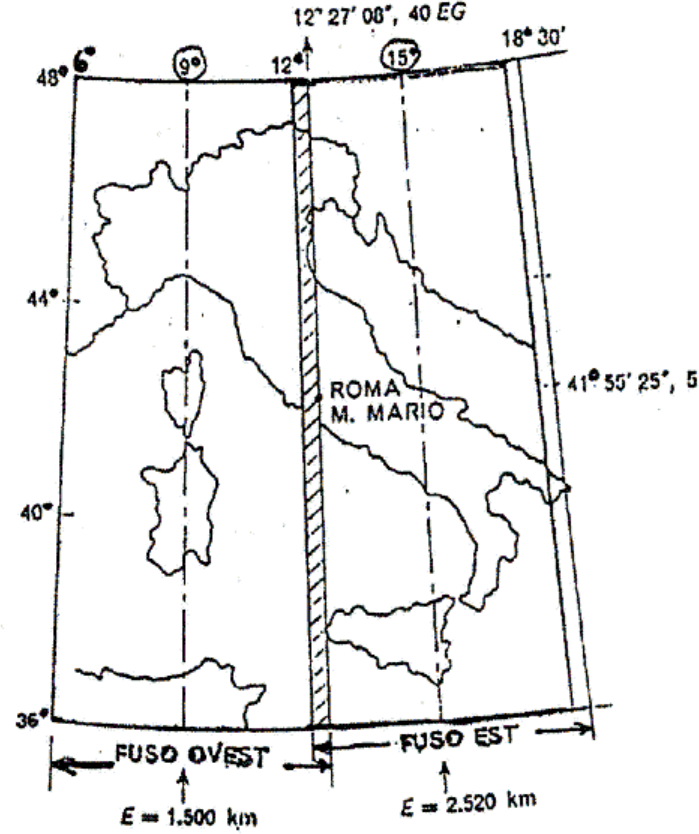
\includegraphics[width=1\textwidth] {./pics/GB.png}
			\end{center}	
		\end{column}		
	\end{columns}
\end{frame}

\begin{frame}
	\frametitle{ER oggi}
	La Regione Emilia-Romagna ha indicato le modalità di condivisione dei dati topografici e cartografici tra Enti, tramite un atto di indirizzo e di coordinamento tecnico con la \textit{legge regionale 20/2000 (articolo 27)}.
	[...]
	%Tra le regole tecniche indicate per l’interscambio dei dati, particolare importanza rivestono proprio le regole di congruenza della georeferenziazione dei dati territoriali e il sistema di riferimento geodetico. 
	L’adozione di un unico sistema di riferimento rappresenta infatti uno dei presupposti per la fruibilità e lo scambio dati territoriali tra le pubbliche amministrazioni centrali, regionali e locali.
	
	Attualmente la Regione si sta preparando ad adottare il sistema di riferimento ETRF2000 (ETRS89) quale sistema principale per le basi dati geotopografiche e per l’interscambio di dati a essa correlati. [...]%L'ETRF2000 è proposto dal Comitato per le regole tecniche dei dati territoriali della Pubblica amministrazione quale sistema di riferimento geodetico nazionale.
	
	Dal punto di vista pratico, in relazione ai sistemi informatici che trattano i dati territoriali, \textbf{il sistema adottato è denominato: ETRS89 / UTM Zone 32N (codice EPSG:25832)}.
	
\end{frame}

\begin{frame}
	\frametitle{ER in passato: UTMA e UTMRER}
	In passato non sempre è stato così, in particolare R.E.R. ha usato proiezioni specifiche prima del datum ED50, poi Roma40 Monte Mario. Nella fattispecie, storicamente si possono individuare 2 sistemi denominati: 
	\small
	\begin{itemize}
		\item \textbf{UTMA} (attualmente in disuso) che nasce come traslazione del SRS ED50-UTM fuso 32 con false origini  di 500000 EST e -4000000 NORD
		%	\begin{center}
		%	 \textit{+proj=tmerc +lat\_ 0=0 +lon\_ 0=9 +k=0.9996 +x\_ 0=500000 +y\_ 0=-4000000 +ellps=intl +units=m +no\_ defs}
		%	 \end{center} 
		E' un sistema  storicamente privo di codice EPSG individuato dai SW ESRI con il  codice 202032 o internazionalmente dal codice 7386 (o 7387) \href{http://spatialreference.org/ref/sr-org/7386/}{\textcolor{gter}{\emph{spatialreference.org}}} 
		\item \textbf{UTMRER} è invece una traslazione del SRS Roma40 Monte Mario con proiezione Gauss-Boaga F. Ovest con false origini  di 500053 EST e -3999820 NORD 
		Per quanto non considerato più come Sistema di riferimento ufficiale regionale, è ancora in uso e \textbf{dotato di un codice EPSG ufficiale 5659} oltre che dal codice interno dei SW ESRI (202003).
		
		
		%	\begin{center}
		%	 \textit{+proj=tmerc +lat\_ 0=0 +lon\_ 0=9 +k=0.9996 +x\_ 0=500053 +y\_ 0=-3999820 +ellps=intl +towgs84=-104.1,-49.1,-9.9,0.971,-2.917,0.714,-11.68 +units=m +no\_defs}
		%	 \end{center} 
	\end{itemize}
	
\end{frame}

\begin{frame}
	\frametitle{UTMA e UTMRER}
	Sembra tutto piuttosto complesso, ma occorre a questo punto sottolineare che \textbf{UTMRER dal punto di vista del valore numerico delle coordinate è assolutamente identico all’UTMA}, in sostanza quindi occorre semplicemente abbinare un SRS UTMRER ai propri archivi da convertire.
\end{frame}

\begin{frame}
	\frametitle{Conversione di coordinate per l'ER}
	\begin{itemize}  
		\item Essendo il caso dell'Emilia Romagna piuttosto specifico, la Regione fornisce attraverso il proprio portale cartografico un SW denominato \textbf{ConvER3\textunderscore 2013}, derivazione di \textit{Convergo}, che serve per le trasformazioni di coordinate fra i vari sistemi includendo i casi specifici regionali. 
		\item I grigliati in formato ntv2 sono inoltre disponibili sia su sistemi ESRI che su SW Open Source come QGIS e precaricati in un opportuno plugin
		\item Avendo a disposizione i codici EPSG dei vari SRS si possono effettuare le conversioni di coordinate direttamente con SW GIS (es. QGIS) con approssimazioni planimetriche di circa 2 m. 
	\end{itemize}   	
\end{frame}

\begin{frame}
	\frametitle{Il Veneto}
	Il Veneto è una delle prime regioni Italiane ad adeguarsi a quanto richiesto dall'IGM. 
	Tutti i dati Veneti dovrebbero essere distribuiti con il sistema di riferimento ufficiale Veneto che è l'\textbf{ETRF2000 (RDN2008) - Fuso 12} (EPSG 7795).
	Sfortunatamente non tutti i SW GIS lo supportano appieno, mentre non c'è nessun tipo di problema ad utilizzare SW open source come QGIS o PostGIS. 	
\end{frame}

\begin{frame}
	\frametitle{Conversione di coordinate per il Veneto}
	\begin{itemize}  
		\item Essendo anche il caso del Veneto piuttosto specifico vista l'adozione del Fuso 12, la Regione fornisce attraverso il proprio portale cartografico un SW denominato \textbf{Conve2014}, derivazione di \textit{Convergo}, che serve per le trasformazioni di coordinate fra i vari sistemi includendo i casi specifici regionali.  
		\item Avendo a disposizione i codici EPSG dei vari SR si possono effettuare le conversioni di coordinate direttamente con SW GIS (es. QGIS) con approssimazioni planimetriche di circa 2 m (per molte scale di lavoro più che sufficienti). 
	\end{itemize}   	
\end{frame}

\section{Trasformazioni fra Sistemi di Riferimento}

\begin{frame}
	\frametitle{Libreria PROJ}
	\setbeamercolor{uppercol}{fg=white,bg=gter}
	\footnotesize
	Infine la \href{https://proj.org/}{Cartographic Projection Library (PROJ)}
    è una libreria per le proiezioni cartografiche su cui si appoggiano i principali GIS FOSS per la trasformazione di coordinate e proiezione rilasciata anch'essa con licenza Open Source MIT.
	\begin{center}
		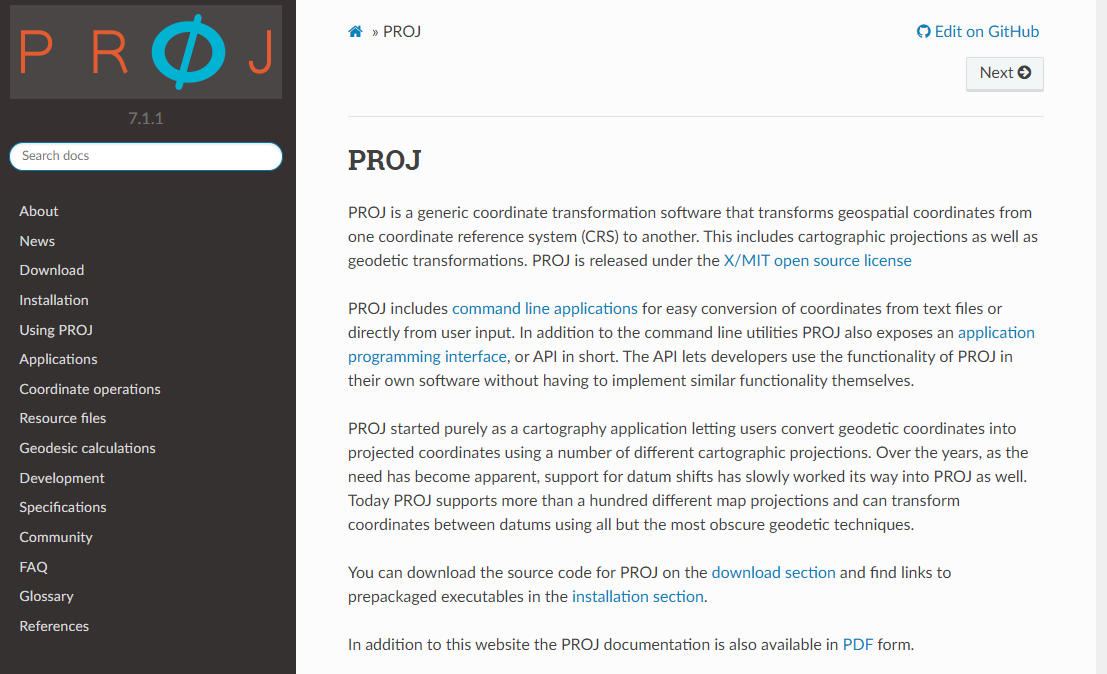
\includegraphics[width=0.7\textwidth]{pics/proj.PNG}
	\end{center}
	
\end{frame}

\begin{frame}
\frametitle{Trasformazioni fra CRS [1]}
 \begin{columns}	
	\begin{column} {0.1\textwidth}
			
\includegraphics[width=1\textwidth] {./pics/worried-bill.png}
	\end{column}
	\begin{column} {0.9\textwidth}
		Con tutti questi sistemi di riferimento, come mi posso comportare?
	\end{column}
\end{columns}
\begin{itemize}
	\item All'interno dei SW GIS si possono gestire complesse operazioni di roto-traslazioni sulla base dei parametri definiti attraverso i codici EPSG. Queste operazioni sono in genere valide su ampie aree (es. tutto il territorio nazionale) e portano ad imprecisioni dell'ordine metrico che, per la maggior parte dei dati territoriali sono inferiori all’errore di graficismo. La libreria PROJ usa dei parametri chiamati \textbf{+towgs84}
	%Uno dei metodi più diffusi per trasformare le coordinate da un sistema geodetico ad un altro è quello della trasformazione conforme 3D, detta anche trasformazione per similitudine, in cui i parametri che consentono di realizzare il passaggio tra i due diversi datum sono in numero di sette, a ciascuno dei quali può essere attribuito un ben determinato significato geometrico2. Tali parametri sono utilizzati nell’ambito dei metodi di trasformazione supportati dall’EPSG (European Petroleum Survey Group) per il passaggio al datum WGS84 come valori del parametro “towgs84”, implementato in QGIS.

\end{itemize}
\end{frame}

\begin{frame}
	\frametitle{Trasformazioni fra CRS [2]}
	\begin{itemize}
		\item Al crescere della scala del dato diventa importante assicurare precisioni più elevate. In questi casi esistono le cosiddette materializzazioni dei sistemi di riferimento a partire dalle quali l’IGM mette a disposizione i cosiddetti \textbf{grigliati}. In questo caso la libreria proj sostituisce il precedenti parametri towgs84 con \textbf{+nadgrids} per le trasformazioni planimetriche.
	\end{itemize}
\end{frame}

\begin{frame}
\frametitle{Grigliati [1]}
Si tratta di griglie a passo regolare che contengono le differenze, espresse in coordinate geografiche, fra i vari sistemi di coordinate e consentono in tal modo di correggere i normali algoritmi di trasformazione.
\\ \vspace{10pt}
La componente altimetrica, quando parte della componente geometrica del dato numerico, è anch’essa trattata attraverso apposite griglie che contengono i valori delle separazioni fra geoide nazionale e l’ellissoide GRS80 di trasformare le quote ellissoidiche in quote ortometriche (o geoidiche, o più comunemente \textit{sul livello del mare}).
\\ Ad oggi l’IGM dispone di due modelli di geoide ITALGEO99 e ITALGEO2005
\end{frame}

\begin{frame}
\frametitle{Grigliati [2]}
L'IGM distribuisce pertanto 3 tipi di grigliati:
\begin{itemize}
	\item Grigliato \textbf{GK1} che integra il modello di geoide ITALGEO99 (file in formato .\textit{gk1});
	\item Grigliato \textbf{GK2} che integra il modello di geoide ITALGEO2005 (file in formato .\textit{gk2});
	\item Grigliato \textbf{NTv2} che consente trasformazioni solo planimetriche (file in formato .\textit{gsb}).
\end{itemize}
\end{frame}

\begin{frame}
\frametitle{SW per conversione che usino i grigliati gk1 e gk2}
\begin{itemize}
	\item L'IGM distribuisce \textbf{Verto2K} e \textbf{Verto3K} (entrambi a pagamento)
	\item Il CISIS (Centro Interregionale per i Sistemi Informatici Geografici e Statistici) distribuisce l'applicazione gratuita \textbf{Convergo} che è poi personalizzata da alcune regioni (es. Veneto, ER, etc)
	\item il Ministero dell'Ambiente anni fa ha realizzato l'applicativo gratuito \textbf{Traspunto} 
	\item 
\end{itemize}
\end{frame}

\begin{frame}
\frametitle{Applicazioni online}
\begin{itemize}
\item anni fa l'\href{https://ww.igmi.org}{IGM} ha realizzato \href{http://212.77.67.76/vol/index_file.php}{Verto online} basato sui grigliati NTv2 (non è aggiornatissimo)
\begin{center}
	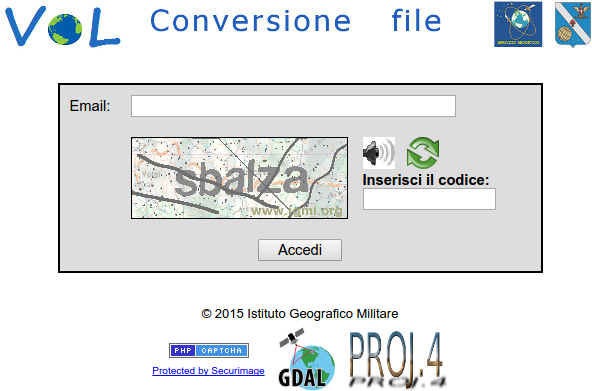
\includegraphics[width=0.5\textwidth]{pics/verto_online.png}
\end{center}
\item il Ministero dell'Ambiente così come alcuni portali cartografici regionali mettono a disposizione geoservizi per la trasformazione di coordinate utilizzando i grigliati
(ma non semplicissimi da utilizzare per l'utente medio)
\end{itemize}
\end{frame}

\begin{frame}
\frametitle{Grigliati e QGIS}
\begin{columns}	
	\begin{column} {0.5\textwidth}
		Alcuni SW GIS, tra questi QGIS e PostGIS, consentono l'utilizzo dei grigliati in formato standard NTv2 per effettuare le trasformazioni di coordinate con i grigliati definendo nuovi sistemi di riferimento.
	\end{column}		
\begin{column} {0.5\textwidth}
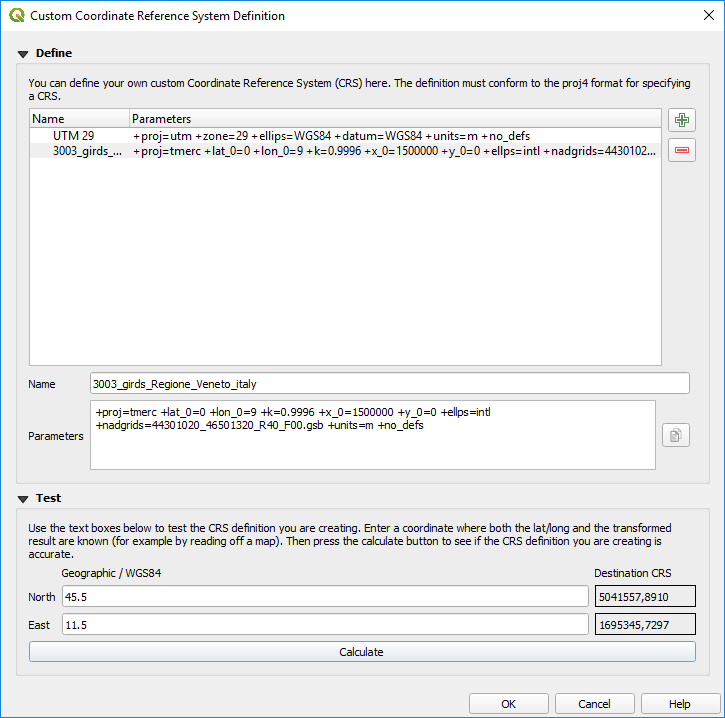
\includegraphics[width=1\textwidth] {./pics/grigliati.png}	
\end{column}		
\end{columns}		
\end{frame}


\begin{frame}
	\frametitle{Grigliati e QGIS}
	I passi da fare se volessi convertire un dato per passare da Roma40 a ETRS sono i seguenti:
	\begin{enumerate}
		\item copiare i grigliati nelle cartelle di sistema (es. $ C:\setminus OSGeo4W64\setminus share\setminus proj $)
		\item definire un nuovo sistema di riferimento in QGIS che usi i grigliati (parametro \textbf{+nadgrids}) da usare come sistema di partenza (es per passare da Roma40 a ETRS usare i file che terminano con R40\_ F00.gsb)
		\item modificare il sistema di riferimento del layer da convertire
		\item esportare il layer usando il sistema di riferimento in cui si vuole convertire il dato 
	\end{enumerate}

    \begin{block}{}
    Per test è possibile anche scaricare in rete presso il sito \href{https://www.globogis.it/?q=download/grigliati-ntv2-litalia}{www.globogis.it} grigliati per tutto territorio
    nazionale rilasciati sotto licenza Creative Commons 3.0 (gratis!!) ma previa
    registrazione.
    \end{block}

\end{frame}

\section{Saluti}

\subsection{Contatti e licenze}
{
\setbeamertemplate{footline}{} 
\setbeamertemplate{headine}{} 
\frame{	
\addtocounter{framenumber}{-1}  % non conto questa slide
\begin{center}
\bigskip

\includegraphics[width=0.2\textwidth]{./Gter.png} \\ 
\scriptsize{
%Gter srl Innovazione in Geomatica Gnss e Gis\\
Via Jacopo Ruffini 9/1A\\
16128 Genova\\
%formazione@gter.it\\
}
\normalsize
\bigskip
\href{www.gter.it}{\textcolor{gter}{\emph{www.gter.it}}}
	
\bigskip	

  	\href{https://twitter.com/@gteronline} { 
\includegraphics[width=0.15\textwidth]{./tw.jpg}}
	\hspace{30pt}
	 \href{http://www.facebook.com/Gteronline} { 
\includegraphics[width=0.15\textwidth]{./fb.jpg}}
	 %\hspace{30pt}
	 %\href{ https://plus.google.com/+GterIt/posts} { \includegraphics[width=0.15\textwidth]{../go.png}}
	 \hspace{30pt}
	 \href{http://www.linkedin.com/company/gter-srl-innovazione-in-geomatica-gnss-e-gis} { 
\includegraphics[width=0.15\textwidth]{./ln.png}}
	 
	 
	 

	 
\bigskip
\vspace{30pt}

	
	\href{http://creativecommons.org/licenses/by-sa/3.0/deed.it} {	
	
\includegraphics[width=0.15\textwidth]{./88x31.png} 
	\\	
	\tiny Quest' opera è distribuita con licenza Creative Commons Attribuzione - Condividi allo stesso modo 3.0 Unported.} 	
	
	
	
\end{center}
%\tableofcontents[pausesections,part=2]
}
}


\end{document}
